%%%%%%%%%%%%%%%%%%%%%%%%%%%%%section Excitation signal setup %%%%%%%%%%%%%%%%%%%%%%%%%%%%%%%%%%%%%%%%%%%%%%%%%%%%%%%%%%%%
%%%%%%%%%%%%%%%%%%%%%%%%%%%%%%%%%%%%%%%%%%%%%%%%%%%%%%%%%%%%%%%%%%%%%%%%%%%%%%%%%%%%%%%%%%%%%%%%%%%%%%%%%%%%%%%%%%
\section{Excitation signal setup} \label{sec:FDTD_Excitation}
An excitation  is a source of the  electric magnetic field. It can be  simulated by an electrical field intensity $\vec{E}$ or a magnetic field intensity $\vec{H}$. In OpenEMS, each excitation can be considered as a composition  of two parts -- a signal of  time (or  frequency) as well as  a geometrical distribution  in the space. The first part is called excitation signal here.
In Matlab this signal is defined as a field of the structure \matv{FDTD}, which is named as \matv{Excitation}. \phantomsection \label{para:Excitation}%\matv{Excitation}

This section will show how to set up  an \matv{Excitation} using different signal, such as a Gaussian pulse, a sinusoidal signal or other custom excitation signal\footnote{How to apply the \matv{Excitation}  to geometrical distribution in the space  is showed in the section \ref{sect-Primitives}.}:
       \begin{myindentpar}
	     \ref{subsec:Gaussian pulse} \hspace{1cm} \hyperref[subsec:Gaussian pulse]{\textcolor{blue}{\underline{\texttt{FDTD=SetGaussExcite(FDTD,f0,fc)}}}}, \\
	      \ref{subsec:Sinusoidal signal} \hspace{1cm} \hyperref[subsec:Sinusoidal signal]{\textcolor{blue}{\underline{\texttt{FDTD=SetSinusExcite(FDTD,f0)}}}},\\
	      \ref{subsec:Other excitation signals} \hspace{1cm} \hyperref[subsec:Other excitation signals]{\textcolor{blue}{\underline{\texttt{FDTD=SetCustomExcite(FDTD,f0,funcStr)}}}}.
       \end{myindentpar}
Note that Gaussian and sinusoidal excitation can be  defined in frequency domain in the above functions, because signals in time domain or frequency domain can be transformed into each other.\\
\info{One  simulation uses only one excitation signal.
If many excitation signals are involved during a simulation, superposition principle can be utilized to  attain the equivalent simulation.}
%%%%%%%%%%%%%%%%%%%%%%%%%%%%%%%%%% subsection Gaussian pulse %%%%%%%%%%%%%%%%%%%%%%%%%%%%%%%%%%%%%%%%%%%%%%%%
    \subsection{Gaussian pulse} \label{subsec:Gaussian pulse}
If $f_0$ is a modulated frequency and $f_c$ is a bandwidth  from   $f_0-0.5f_c$ to  $f_0+0.5f_c$ where the excitation amplitudes  are greater than $-5$dB, a time domain Gaussian signal (Indeed it's a pure Gaussian signal modulated by a co-sinusoidal signal. See fig. \ref{fig:GaussInpulseTheory})
\begin{equation}\label{equ:GussianSignal_time}
 f(t)=cos[2\pi f_0(t-t_0)]e^{-{\big(\frac{t-t_0}{\frac{t0}{3}}\big)}^2}, \quad \text{for } t>0 \text{ and }t_0=\frac{9}{2\pi f_c}
\end{equation}
can be transformed  into frequency domain as
\begin{equation}\label{equ:GussianSignal_freq}
F(f)=\frac{3}{4\sqrt{\pi}f_c}e^{-j\frac{9f}{f_c}}e^{-{\big(\frac{f-f_0}{\frac{2f_c}{3}}\big)}^2},\quad \text{for } f>0 .
\end{equation}

Figure \ref{fig:GaussInpulseTheory} shows an instance of Gaussian pulse from expressions \ref{equ:GussianSignal_time} and \ref{equ:GussianSignal_freq}. 
    \begin{figure}[hbt]
	      \centering
	      \subfloat[In time domain]{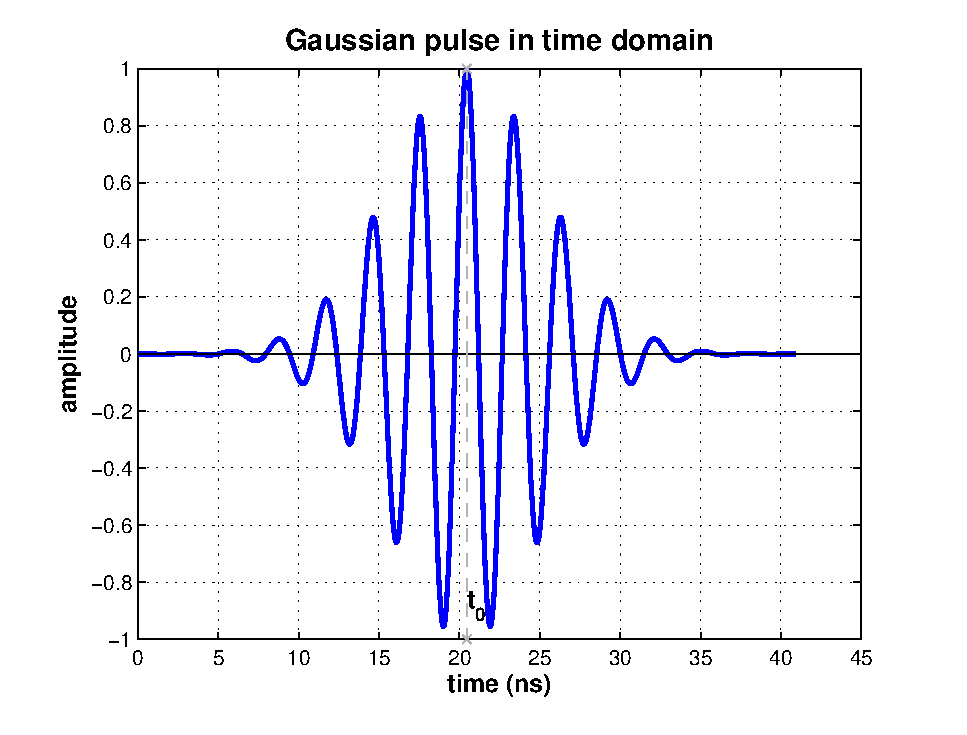
\includegraphics[width=0.48\textwidth]{svg/GaussPulseTime.eps}} 
	      \subfloat[In frequency domain]{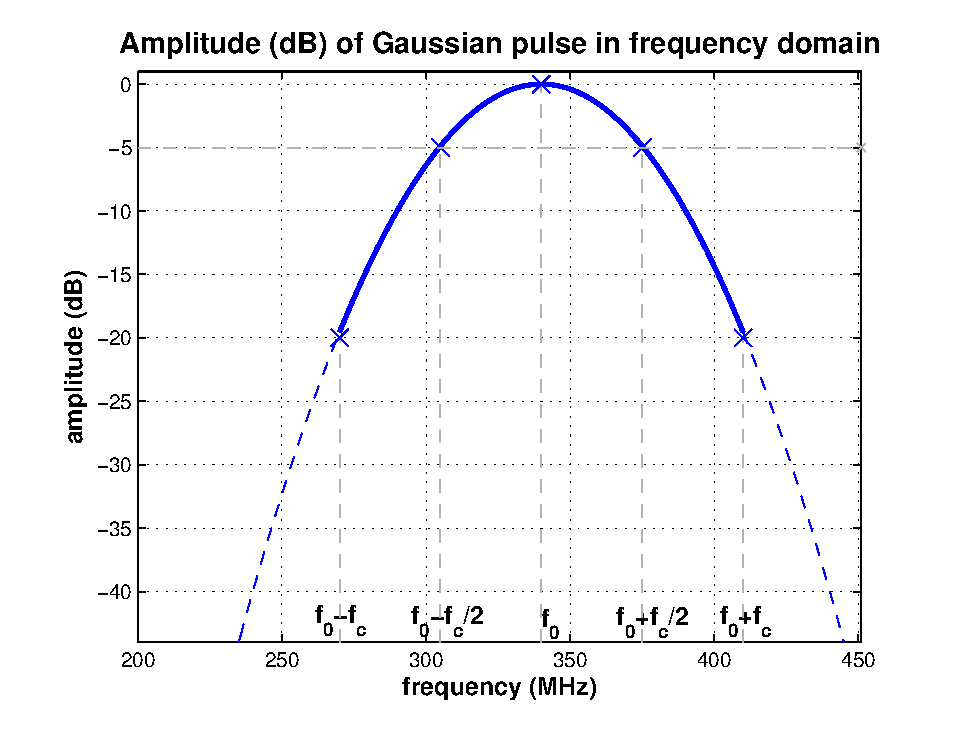
\includegraphics[width=0.48\textwidth]{svg/GaussPulseFreq.eps}}
	      \caption[Gaussian pulse signal]{An instance of Gaussian pulse signal with $f_0=340$ MHz $f_c=70$ MHz}
	      \label{fig:GaussInpulseTheory}
    \end{figure}
According to the expression \ref{equ:GussianSignal_freq}, a Gaussian signal can be defined using function \hyperref[func:SetGaussExcite]{\texttt{SetGaussExcite()}}.

%%%%%%%%%%%%%%%%%%%%%%% FUNCTION  SetGaussExcite %%%%%%%%%%%%%%%%
\begin{FontNameFunct}{SetGaussExcite()}
\phantomsection \label{func:SetGaussExcite}
\end{FontNameFunct}

%%%%%%%%%%%%%%%%%%%%%%%%%%%% Purpose
\begin{FontDescr}{Purpose:}
 Set  Gaussian function (eq.\ref{equ:GussianSignal_freq}) as  signal of an excitation.  
\end{FontDescr}

%%%%%%%%%%%%%%%%%%%%%%%%%%%% Syntax	  
\begin{FontDescr}{Syntax:}
      \begin{lstlisting}
FDTD = SetGaussExcite(FDTD,f0,fc)
      \end{lstlisting}
\end{FontDescr}

%%%%%%%%%%%%%%%%%%%%%%%%%%%% Description
\begin{FontDescr}{Description:}
    %%%%%%%%%%%%%%%%%%%%%%%%%%%% f0
    \begin{FontPara}{f0} \phantomsection \label{para:f0}
   \matv{f0}  is the frequency of the modulating co-sinusoidal signal. It's also the central frequency of the Gaussian signal. With \matv{f0} the signal has the highest amplitude or energy.
    \end{FontPara}
    %%%%%%%%%%%%%%%%%%%%%%%%%%%% fc
    \begin{FontPara}{fc} \phantomsection \label{para:fc}
		\matv{fc} determines the variance of the signal. It is a  bandwidth of which center is at \matv{f0}. In the band [\matv{f0}-0.5\matv{fc} \quad \matv{f0}+0.5\matv{fc}] the amplitude  is greater than  $-5$dB (See fig. \ref{fig:GaussInpulseTheory}).
% The maximal frequency which will be simulated is \matv{f0}+\matv{fc}.
The broader \matv{fc} is, the less steep is the signal in frequency domain, but narrower  and steeper the signal is in time domain.
    \end{FontPara} 
\end{FontDescr}

\warning{ Small \matv{fc} for narrow band will lead to a time-consuming simulation. Great \matv{fc} for broadband will lead to a  signal  in short time. }

%%%%%%%%%%%%%%%%%%%%%%%%%%%% Examples
\begin{FontDescr}{Examples:}
 \begin{itemize}
\item A Gaussian pulse with a central frequency \matv{f0}=$340$ MHz and a  bandwidth of \matv{fc}=$70$ MHz in which the amplitude is greater than $-5$ dB.
\begin{lstlisting}
% Initiation of FDTD. Maximal number of time step is 5000. End criteria of energy is -50 dB.
FDTD = InitFDTD(5000,1e-5,'OverSampling',10);
% Update FDTD with a  Gaussian pulse excitation.
% f0=340 MHz, fc=70 MHz
FDTD = SetGaussExcite(FDTD,340e6,70e6);
% The field  FDTD.Excitation.ATTRIBUTE  has been assigned.
\end{lstlisting}
Under this setting, an excitation signal of Gaussian pulse has been set up. The signal reduces to $-5$ dB at $305$ MHz or $375$ MHz (to $-20$ dB at $270$ MHz or $410$ MHz).
\end{itemize}
\end{FontDescr}

%%%%%%%%%%%%%%%%%%%%%%%%%%%%%%%%%%%% subsection Sinusoidal signal %%%%%%%%%%%%%%%%%%%%%%%%%%%%%%%%%%%%%%%%%%%%%%%%%%%%%%%%%%%%%%%%%%%%%
    \subsection{Sinusoidal signal}\label{subsec:Sinusoidal signal}
%%%%%%%%%%%%%%%%%%%%%%% FUNCTION  SetSinusExcite %%%%%%%%%%%%%%%%
\begin{FontNameFunct}{SetSinusExcite()}
\phantomsection \label{func:SetSinusExcite}
\end{FontNameFunct}

%%%%%%%%%%%%%%%%%%%%%%%%%%%% Purpose
\begin{FontDescr}{Purpose:}
 Set a sinusoidal function as the signal of an excitation.
\end{FontDescr}

%%%%%%%%%%%%%%%%%%%%%%%%%%%% Syntax
\begin{FontDescr}{Syntax:}
      \begin{lstlisting}
FDTD = SetSinusExcite(FDTD,f0)
      \end{lstlisting}
\end{FontDescr}

%%%%%%%%%%%%%%%%%%%%%%%%%%%% Description
\begin{FontDescr}{Description:}
       The signal in time domain has a form as following function\\
\begin{equation}\label{equ:SinusoidalSignal_time}
 f(t)=\sin{(2\pi f_0t)}, \text{ for } t>0
\end{equation}
    %%%%%%%%%%%%%%%%%%%%%%%%%%%% f0
    \begin{FontPara}[para:sinf0]{f0} \phantomsection \label{para:sinf0}
   \matv[para:sinf0]{f0}  is the unique frequency of the  sinusoidal signal.
    \end{FontPara}
\end{FontDescr}

%%%%%%%%%%%%%%%%%%%%%%%%%%%% Examples
\begin{FontDescr}{Examples:}
 \begin{itemize}
\item A sinusoidal signal with a  frequency \matv[para:sinf0]{f0}=0.5 GHz.
\begin{lstlisting}
% Initiation of FDTD
FDTD = InitFDTD(5000,1e-5,'OverSampling',10);
% Assignment for f0
f0=0.5e9;
% Update FDTD with a sinusoidal excitation.
FDTD = SetSinusExcite(FDTD,f0);
% The field  FDTD.Excitation.ATTRIBUTE has been assigned.
\end{lstlisting}
A sinusoidal excitation with frequency $0.5$ GHz has been set up for simulation in OpenEMS.
\end{itemize}
\end{FontDescr}


%%%%%%%%%%%%%%%%%%%%%%%%%%%%%%%%%%%% subsection Other excitation signals %%%%%%%%%%%%%%%%%%%%%%%%%%%%%%%%%%%%%%%%%%%%%%%%%%%%%%%%%%%%%%%%%%%%%
    \subsection{Other excitation signals}\label{subsec:Other excitation signals}
OpenEMS provides various kinds of excitation signals. Besides the Gaussian pulse and sinusoidal signal, it has other forms of signal, such as Dirac function, step function and even custom function. Here is the introduction of how to set up an excitation with any custom function by using \hyperref[func:SetCustomExcite]{\texttt{SetCustomExcite}}.

%%%%%%%%%%%%%%%%%%%%%%% FUNCTION  SetCustomExcite %%%%%%%%%%%%%%%%
\begin{FontNameFunct}{SetCustomExcite()}
\phantomsection \label{func:SetCustomExcite}
\end{FontNameFunct}
	  
%%%%%%%%%%%%%%%%%%%%%%%%%%%% Purpose
\begin{FontDescr}{Purpose:}
Set a custom function as the signal of the excitation.
\end{FontDescr}

%%%%%%%%%%%%%%%%%%%%%%%%%%%% Syntax
\begin{FontDescr}{Syntax:}
      \begin{lstlisting}
FDTD = SetCustomExcite(FDTD,f0,funcStr)
      \end{lstlisting}
\end{FontDescr}
      
%%%%%%%%%%%%%%%%%%%%%%%%%%%% Description
\begin{FontDescr}{Description:}
       The signal in time domain is defined using a  custom function which is given in the form of a string \matv{funcStr}.
    %%%%%%%%%%%%%%%%%%%%%%%%%%%% f0
    \begin{FontPara}[para:customf0]{f0} \phantomsection \label{para:customf0}
   \matv[para:customf0]{f0}  is the nyquist rate.
    \end{FontPara}
    %%%%%%%%%%%%%%%%%%%%%%%%%%%% funcStr
    \begin{FontPara}{funcStr} \phantomsection \label{para:funcStr}
      \matv{funcStr}   is a string of an expression in MATLAB. This expression is of time \texttt{t}.  Two constants can be used directly in the expression, \texttt{e} for Euler's number and \texttt{pi} for $\pi$. Furthermore, any strings of defined variables can be used in the  string \matv{funcStr} for the expression of the signal.
    \end{FontPara}
\end{FontDescr}

%%%%%%%%%%%%%%%%%%%%%%%%%%%% Examples
\begin{FontDescr}{Examples:}
    \begin{itemize}
	\item A ramped sinus excite
	\begin{lstlisting}
% Initiation of FDTD
FDTD = InitFDTD(5000,1e-5,'OverSampling',10);
% The nyquist rate f0=1GHz
f0=1e9;
% Time step is of the nyquist rate f0
T = 1/f0;
% Update FDTD with a given string
% of an excitation expression of t.
FDTD = SetCustomExcite(FDTD,f0, ...
       [ '(1-exp(-1*(t/' num2str(T) ...
        ')^2) ) * sin(2*pi*'  ...
        num2str(f0) '*t)' ]);
% The field  FDTD.Excitation.ATTRIBUTE
% has  been assigned.
	\end{lstlisting}
\end{itemize}
\end{FontDescr}
